\section{Recommendation Systems in Software Engineering}



Software development is a challenging and knowledge-intensive activity. It 
requires mastering several programming languages, frameworks, design patterns, 
technology trends (among other aspects) under the pressure of ever-increasing 
arrays of external libraries and resources 
\cite{robillard_recommendation_2014}. Consequently, software developers are 
continuously spending time and effort to understand new third-party libraries, 
existing code or how to properly implement a new feature.  The time spent on 
discovering useful information can have a dramatic impact on productivity 
\cite{Duala-Ekoko:2012:AAQ:2337223.2337255}. 

Over the last few years, a lot of effort has been spent on data mining and 
knowledge inference techniques to develop methods and tools able to provide 
automated assistance to developers in navigating large information spaces and 
giving recommendations that might be helpful to solve the particular 
development problem at hand. The main intuition is to bring to the domain of 
software development the notion of recommendation systems that are typically 
used for popular e-commerce systems to present users with interesting items 
previously unknown to them \cite{Ricci2011}.

Robillard and colleagues define a \textit{Recommendation System in Software 
Engineering (RSSE)} as ``... a software application that provides information 
items estimated to be valuable for a
software engineering task in a given context'' 
\cite{robillard_recommendation_2014}. In particular, when developers join a new 
project, they have to typically master a huge number of information sources 
\cite{Dagenais:2010:MNS:1806799.1806842} (often at a short time). In such a 
context, the problem is not the lack of information but instead an information 
overload coming from heterogeneous and rapidly evolving sources.
Thus, RSSEs aim at giving developers recommendations, which can consist of 
different items including code examples, issue reports, reusable source code, 
possible third-party components that might used, documentation, etc. 

\begin{figure}[h!]
	\centering
	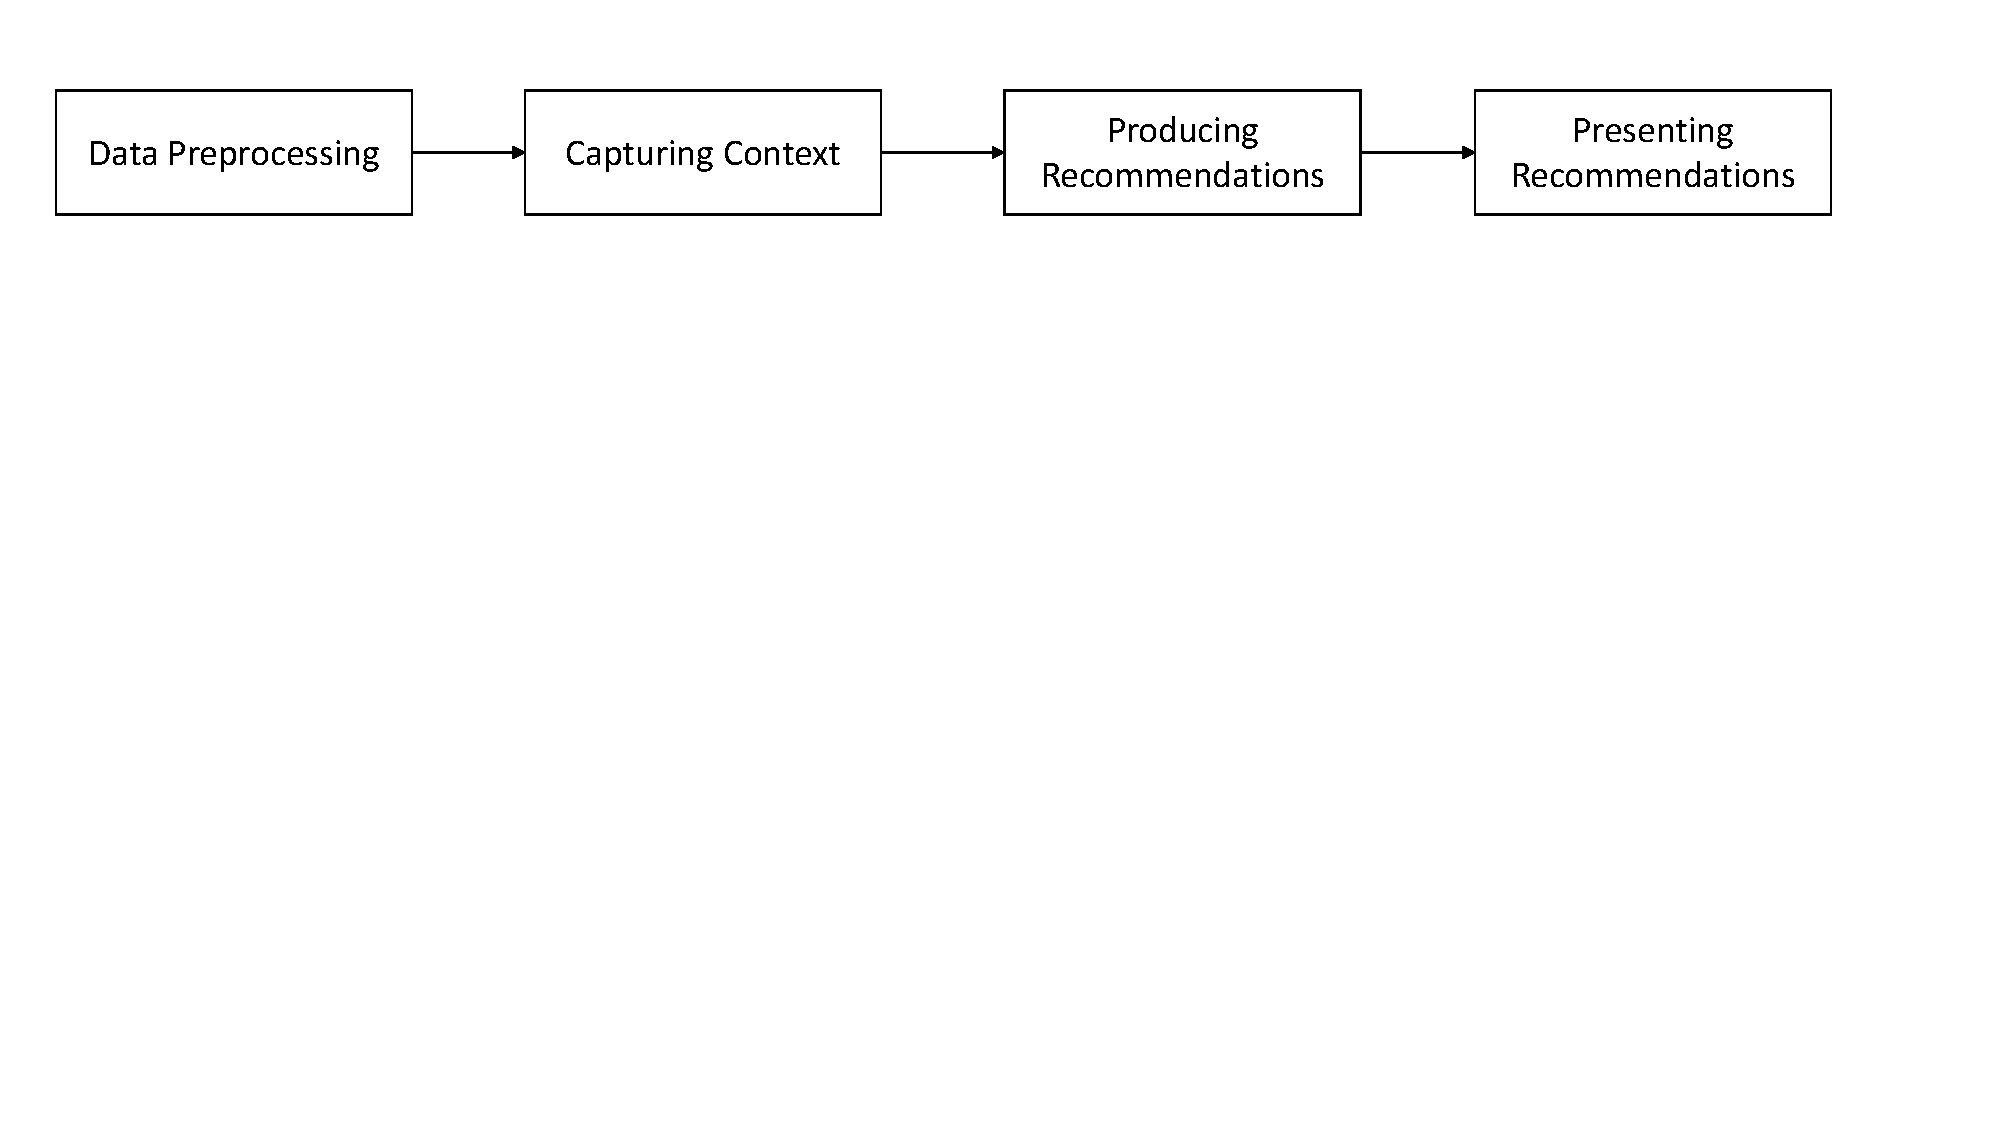
\includegraphics[width=\linewidth]{images/rs-steps}
	\caption{Main RSSEs challenges}
	\label{fig:rs-steps}
\end{figure}

The design and development of a RSSE has to take into account a number of 
challenges including those shown in Fig. \ref{fig:rs-steps} and described below 
\cite{robillard_recommendation_2014}:

\begin{itemize}
	\item[--] \textit{Data Preprocessing:} all the data sources that might 
	contain valuable information for the developer have to be preprocessed in 
	order to be subsequently analyzed. For instance, erroneous data needs to be 
	removed, source code has to be parsed, bug tracker issues have to be 
	analyzed, dependency graphs have to be derived etc.
	\item[--] \textit{Capturing Context:} to conceive recommendations that are 
	really valuable for the developer, it is necessary to capture the user 
	profile, and to properly represent the task the developer is working on. 
	The context can be explicitly specified by the developer or implicitly 
	inferred by the development environment e.g., by analysing the source code 
	being edited, the third-party components used, the issue report that a user 
	is reading, etc. 
	\item[--] \textit{Producing Recommendations:} once data sources have been 
	preprocessed and the developer context has been captured, the 
	recommendation algorithms can be executed.
	\item[--] \textit{Presenting Recommendations:} produced recommendations 
	should be sent to developers and presented in a timely and appropriate way. 
	This means that depending on the task the developer is working on, 
	recommendations can be represented as potential lists of issue reports, 
	source code suggestions, links to Stack Overflow posts, etc. Beyond the 
	recommendation items, developers should be provided also with explanations 
	related to the suggested artifacts, which might be also ranked according to 
	some criteria.
\end{itemize}


CROSSMINER can be seen as a recommendation system aimed at supporting 
developers while producing new software by integrating existing open source 
components. In particular, the \textit{data preprocessing} challenge is 
addressed by the CROSSMINER analysis tools targeting source code, communication 
channels, and configuration specifications. The developer context is captured 
by an Eclipse-based IDE, which also produces recommendations that do not 
require particular and expensive data analysis. For more elaborated 
recommendations, preprocessed data available in a dedicated knowledge base is 
used. Both the IDE and Web based dashboards will be used to present the 
produced recommendations to the developer. 

%
%
%
%First of all, we have to look at definition of recommendation.  In general, a 
%recommendation is a suggestion or a proposal as to the best course of action, 
%often provided by an authoritative body or expert domain. The key concept when 
%we talk about recommendation is the context, because it changes meaning with 
%respect to the type of system that a developer is working in. \\
%We can find recommendation system in software engineering (RSSE) that gives 
%the necessary information about suitable items for a software engineering task 
%in a specific context. When a developer starting to work on a project, there 
%are several information spaces, also called landscape, that describe all 
%involved information in the overall developing process. 
%In~\cite{martin_p.robillard_introduction_2009}, the authors define all 
%possible 
%information spaces in software engineering but this definition can be applied 
%in whatever software complex system. Related to the developed project, the 
%main 
%definition is the project source code and project history, that give the 
%context of developing. The project source code is useful to understand the 
%structure of it, especially when we looking for method declarations, method 
%calls and possible most frequent pattern while the project history tells 
%something about the changing happened in the code from a older version to 
%another. \\
%This changes are usually captured by a VCS (version control system) although 
%this kind of system isn't easily browsable and techniques like data mining or 
%machine learning are required. Development environment also belongs to this 
%information spaces classification and it includes all scripts, commands and 
%tools used to test and run the system. Another big information space is 
%defined 
%by API that are linked to the project as well as their documentation, a good 
%starting point to better understand their behaviours. Moreover, the authors 
%consider also two types of traces when a user is developing a project: 
%interaction traces, composed by the list of user's actions like search on 
%website for particular component or interface and normally this kind of 
%information are captured by an IDE (like Eclipse); the execution trace, 
%instead, regarding the software runtime execution and the collected 
%information 
%are in general function calls and results of computation at every time. 
%Finally, a very important information space is represented by the web that 
%becomes more and more relevant in recent years; in particular, Stack Overflow 
%questions and answers site is the most used by the developers as we can find a 
%lot of concrete example about code snippets as well as information about 
%interfaces, technologies and tools. \\
%As we can see, all this information spaces represent an huge data mine and 
%there are many problems to extract the correct information from it. First of 
%all, the available information are heterogeneous and context awareness while a 
%typical user is looking for a quickly solution related to its specific 
%context. 
%Furthermore, the complex software systems are rapidly growing and it can lead 
%the overload information problem. So, looking at this problem, it is necessary 
%to find a proper way to do recommendation, in the manner that the developer 
%find a good solution in very few time without waste it to search in very large 
%context. For the software engineering context, the authors propose RSSE, a 
%recommendation system for software engineering based on capturing the context, 
%giving the proper recommendation. The process involves some kind of data 
%preprocessing, capturing the context, select the correct recommendation using 
%collaborative filtering techniques and show them to the user.\\
% The first phase involves often effort because includes many type of 
%operations on data like transformation, gathering, filtering, aggregation and 
%so on. The next step is the capture of the context, that is a key issue in a 
%recommendation system. In another domains, like e-commerce for example, the 
%context is strongly related to the user's characteristics and its behaviours; 
%reversely, in the software engineering and in the software domain in general, 
%the recommendation are related to the task that the developer wants to 
%perform. 
%So, in this domain we talk about the task context, that in general a smaller 
%part of the final solution. This kind of systems are called task-centric 
%against the human-centric system in which the recommendations are related to 
%the user. However, the capturing of this context could bring some bias, in 
%particular we could be in the situation in which the context are extremely 
%precise, maybe because we have a lot of information, but the user, especially 
%if he is a not expert domain, doesn't known how to use them or how to provide 
%enough information to describe in the proper way the context. After this 
%preparatory phases, a recommendation algorithm can be executed to produce the 
%final output. The literature is plenty of this techniques that go from the 
%collaborative filtering techniques to similarity matrix, as we will see in 
%next 
%section. Of course, the choice of the algorithm to be used affects the 
%precision, the accuracy and the coverage of the approach, making this task the 
%most important during the development of a recommendation system. The last 
%step 
%is the presenting of the recommendation to the final user. Also in this case, 
%the form of representation depends on the domain in which the recommendation 
%system operates; so, considering the context, we can have a list of function 
%calls, variables, classes as well as documentation or issues reports. Beyond 
%the form of recommendations, a recommendation system must be to classify and 
%rank the results, following a well-formed criteria, such as number of lines, 
%probability, time, average rating and so on. This criteria naturally depends 
%once again on the task context. \newline
%Moving in the context of the IDEs, auto-completion can be a kind of 
%recommendation at runtime because the developer, usually through shortcuts, 
%wants suggestion for specific functions and methods. This technique uses often 
%documentation embedded in the IDE (like JavaDoc in Eclipse) and it adapts 
%itself  to the context, in this case the imported libraries in the project. 
%Moving to a more general definition, we are in the query auto completion (QAC) 
%domain, used in several contexts like search engine, as described 
%in~\cite{DBLP:journals/ftir/CaiR16}.\\
%It is a particular form of word prediction: when a user is typing something, 
%such as fragment of code,method declaration or just first characters, QAC 
%completes the query using different techniques like n-gram technique, 
%probabilistic methodologies and heuristic learning algorithm. Beyond the used 
%technique, QAC system ranks the possible results of a query following a 
%predefined criteria. In case of auto-completion, the query engine maps the 
%prefix, namely the query that the user is writing, to possible list of results 
%and gather all the date in a effective data structure like prefix tree in 
%order 
%to avoid waste of time. Another purpose of a QAC system is try to predict the 
%user's prefix, by retrieving the top rank queries before the entire process is 
%finished. Moving to the possible approaches, there are two main categories: 
%heuristic model and learning-based model. These two category can be divided 
%again into three categories: time sensitive, contextual based and 
%demographic-based. The first is involved when there are time constrains while 
%the contextual and demographic based categories are strongly related to the 
%user's previous history. \newline
%So, we look at the different types of context that a recommendation system 
%must face. Depending on the context, the proposed recommendations change too, 
%sometimes in a radical way. For us, the context are represented by Java 
%projects and in particular, API function call related to external libraries.

\section{Learning APIs: issues and solutions}

An API (Application Programming Interface) is defined as a set of procedures, 
protocols and objects that gives to the developers the necessary building 
blocks to implement a specific functionality. Depending on the context, these 
building blocks can be classes, interfaces and methods properly declared and 
used or intermediate software that acts as middleware in different situations 
as well as in the hardware context. The concept of API is strongly related to 
libraries that a developer uses and the kind of application that he is 
developing. 

APIs can be complex and consequently their usability can be affected. In 
\cite{martin_p._robillard_what_2009} authors analyse the difficulties that can 
raise when developers want to learn and use a given API. In particular, in 
\cite{martin_p._robillard_what_2009} authors considered professional developers 
at Microsoft and try to understand what are the main issues in the API context. 
As starting point, the author of the article asks to a population composed by 
30,000 people among engineers, developers and program manager in the Microsoft 
context. The survey starts with some questions about the developer's skills, to 
asses the knowledge of the participants. Additional questions are defined to 
characterize the problems on learning an API, strongly related to the context, 
familiarity with the application domain, the obstacles faced during the 
learning phase and so on. From the initial population, 83 developers were 
selected and distinguished as expert, and junior. From the answers of such 
developers five obstacle categories were identified with the aim of identifying 
the main problems that the considered developers encountered during the 
learning phase of the used APIs. The category with the more answers is related 
to the obstacles due to the absence or inadequate resources in the learning 
phase, such as not suitable code example, partial information about the content 
of APIs, no reference about the task to perform, inadequate resources format, 
and insufficient high-level design and not well-formed structure of the API. 
Other problems are related to the structure, especially for debugging and 
runtime phases, the developer's background, technical issues and problems that 
arise during the runtime execution.
%
In order to mitigate these issues, the documentation of an API must include 
good examples for the functions and code to develop, the support for case study 
scenarios, good organization of the relevant design elements. 

%Another key point 
%is the context, because the API change often their behaviour depending on it, 
%as pointed out from 12 audio interview that author made with the developers 
%adding their answer to the initial survey. 

In general, APIs follow the so called low barrier to entry, that consists to 
give just few information and key concept about the APIs structure and design, 
sometimes involving basic code examples. Although it is a very spread 
techniques, the survey underlines that is not enough to give a concrete help 
during the learning phase. Many developers involved in the survey, in facts, 
claim that they are often confused about multiple uses of a certain function, 
because there are different approaches to implement a feature but they not 
understand what is the proper one, considering also the context in they are. 
This issue affects also the general structure of the APIs, like the design that 
often generate confusion if it is not well specified and the survey respondents 
want also to understand what are the rationale behind the API. 

Although the abstract design and the overall structure are important when we 
talk about APIs usage, the most immediate and concrete hints are related to 
code example \cite{martin_p._robillard_what_2009}. In particular, the survey 
shows that the Microsoft developers not always understand the examples provided 
in the documentation. Table \ref{tab:ApiCodeExampleCategories} shows the main 
three categories of code examples that could be provide by an online 
documentation or in a general \textit{readme} file of a given API. 

\begin{table}[!t]
  \small
%	\begin{adjustbox}{width=1\textwidth}
		\begin{tabular}{|c|p{9.5cm}|}
			\hline
			 \textbf{Code example category } & \textbf{Description} \\
			\hline
			 Code Snippet & It gives just a flavour of basic concepts of the 
			 API and their possible use\\
			\hline
			Tutorial & It is a quite complete example of a possible use of API, 
			with multiple methods and functions usage\\
			\hline
			Application & It gives a well structured example of the API, given 
			also the development context \\
			\hline
		\end{tabular}
%	\end{adjustbox}
  	\caption{Main categories of code examples available with APIs}
	\label{tab:ApiCodeExampleCategories}
\end{table} 

Looking at these categories, code snippets provide immediate hints but they are 
more related to specific issues, such as opening a connection or initialize a 
particular object. Tutorials provide more complete examples, with different 
methods, often followed by a textual explanation with the aim to show the 
rationale behind the code. The code example coming from the applications, 
instead, wants to give a general overview of the API features and it includes 
demonstration samples and complete open source projects. However, the Microsoft 
developers involved in the survey denoted that usually the code snippet doesn't 
provide how to put together all the small pieces. Another problem is that the 
code examples available from the Web are out-of-date and the maintenance of 
them is still an opening question. In \cite{martin_p._robillard_what_2009}, 
authors list possible improvements related to the code examples, by providing 
best practices in a certain situation, by giving the design behind the code 
example and by showing in a clear way how the considered API works in practice. 
All this information should be inserted in the documentation provided with the 
API. In  \cite{martin_p._robillard_what_2009}, authors claim also that the 
behaviour of a given API can diverge from that described in the documentation 
or from the code examples. 

%%%%%%%%%%%%%%%%%%%%%%%%%%%%%%%%%%%%%%%%%
\smallskip
In~\cite{by_christopher_scaffidi_why_2006} authors identify some 
issues and challenges that developers have to deal with to use and understand 
an API, such as the already mentioned inadequate documentation or the 
inappropriate abstraction in the overall design. Additionally, in 
\cite{by_christopher_scaffidi_why_2006} authors suggest possible workarounds 
for the different situations that the API designers should take into 
consideration. The ideal design flow when a API designer should 
follow includes gathering information from the stakeholders (mainly 
other developers that want to reuse the API functionalities), map the 
requested features to the proper components and set up the glue code to make an 
usable and understandable platform. However, this implies a well specified 
design flow and a lot of time, and sometimes the timing constraints on the 
publication of a new API do not allow to have a complete and exhaustive 
documentation. Even \textit{Hello World} examples might not be enough 
especially if the target user is not an expert of the considered application  
domain. Another potential problem is represented by the orthogonal 
functionalities, also called \textit{internal couplings}. They refer to 
situations when a method is strongly dependent with another one or its 
behaviour can affect other parts of the system. To avoid these situations,  API 
designers have to keep the overall platform as simpler as possible, by limiting 
the exponential growing of the system. 

Concerning the abstraction problem, the users are in the situation in which the 
requirements do not match the proper methods or interfaces provided by the API. 
Such a situation goes beyond a lack of information in the documentation, 
because it is a problem that affects the initial design of the API. A designer 
should set abstractions for each user's requirement, in order to maintain the 
proper mapping and to avoid the loss of functionalities. Another possible 
solution is to use the facade pattern to make more accessible the API itself. 
The last main issue underlined in ~\cite{by_christopher_scaffidi_why_2006}  is 
the external dependencies, called \textit{assumptions}, that an API could 
require to perform a certain operation. For the designer a possible solution 
can be the limitation of external calls to another API, maybe by reusing the 
internal API features. 


All the solutions that authors provide in 
~\cite{by_christopher_scaffidi_why_2006} are inspired by three key concepts: 
\textit{i)} making the addressed problem as smaller as possible, by splitting 
the initial one to little problems that can be solved in less time; 
\textit{ii)} approximating the final solution, by looking first at all to the 
user's requirements with the aim of satisfying them; \textit{iii)} if the 
feature or the functionality to implement is really complex, an API's designer 
should choose an approach that is optimal in the average case. 

%%%%%%%%%%%%%%%%%%%%%%%%%%%%%%%%%%%%%%%%%
\smallskip
As said before, usability plays an important role in API learning. 
In~\cite{marco_piccioni_empirical_2013},  authors focus their attention on this 
problem by performing a human survey. A cognitive framework is proposed to 
evaluate the human reaction that take place when a user is implementing a 
particular feature by means of a given API. This indicator wants to measure 
what is expected during the development and what really happens. With this 
technique, the authors gather the reactions and so the implicit feedback coming 
from the programmers avoiding in this way the bias led by subjective 
perceptions. Of course, the cognitive analysis is combined with the classical 
research question, about the difficulties to learn a new API, the 
understandability of the usage and the abstraction of the overall platform. 
Usability tokens are also extracted from the interviews to measure different 
developer's behaviours in different situations. Here below there are the list 
of tokens used in the questionnaire:

\begin{itemize}
	\item \textit{surprise}: it measures the unexpected behaviour of a 
	particular component of the API, that seemed different at the beginning;
	\item \textit{choice}: it evaluates the capacity of the developer to 
	understand what is the optimal solution for solving a particular problem, 
	like use the proper data structure;
	\item \textit{missed}: it belongs to the abstraction problem, when the 
	developer loses something because she does not understand the API design;
	\item \textit{incorrect}: in this case, the developer uses in the wrong way 
	the provided function or classes;
	\item \textit{unexpected}: this token describes the situation in which the 
	user takes decisions that are not documented by the API's designer.
\end{itemize}

The usability tokens are strongly related to the cognitive dimensions and they 
can be combined to depict a particular situation in which some obstacles occur 
at the same time. The experiment is overtaken on ABEL, an object oriented 
library for storing and retrieving huge amount of information. The results of 
this empirical study, that involves heterogeneous group of developers, show 
that the critical issue is to understand the relations between types and 
classes, not always understood by the participants. Other minors issues are the 
incorrect usage of the provided interfaces or the treatment of constructors 
without arguments, but in those cases the developers are able to overshoot 
these issues. 

Overall, according to the studies mentioned above, understanding and using 
third-party APIs can be very challenging. Consequently, advanced techniques and 
tools are needed to automatically mine APIs with the aim of supporting 
developers during their adoption as presented in the next chapter.
